\documentclass{article}

% Math packages
\usepackage{amsmath}
\usepackage{amssymb}
\usepackage{float}

% R Table packages
% booktabs and float are used frequently by kableExtra output from R
\usepackage{booktabs}
\usepackage{float}
\usepackage{colortbl}
\usepackage{xcolor}

% Page layout libraries
\usepackage{a4wide}
\usepackage{setspace}
\usepackage{geometry}
%\usepackage{parskip}
\usepackage{fancyhdr}
\usepackage{natbib}

% Setting up the heading style preferred here
\pagestyle{fancy}
\fancyhead[L]{\thepage}
\fancyhead[C]{}
\fancyhead[R]{\textrm{Robert Petit}}
\fancyfoot[L, C, R]{}


% this package helps us with including images. Setting the graphics path makes it easier to refer to things in the \includegraphics command.
\usepackage{graphicx}
\graphicspath{ {../Figures/} }

% And finally, continuing on my crusade to make Helvetica the universal standard
\usepackage[scaled]{helvet}
\renewcommand\familydefault{\sfdefault} 
\usepackage[T1]{fontenc}

% Titling
\title{Gateway To Sobriety \\
    \large The Impact of Marijuana Legalization on Alcohol, Cocaine, and Heroine}
\author{Robert Petit}
\date{May 2022}

\begin{document}
\maketitle

\begin{abstract}
    Starting in 2012, the legalization of marijuana for recreational began in Colorado and Washington. The effect of these laws is of great interest and debate. In this study, we construct a synthetic control study to investigate the impact of this law in Colorado on admission rates into treatment programs for drug abuse. We utilize SAMHSA TEDS-A data set and census data in order to estimate the causal treatment effect on the treated group (Colorado) in terms of the rate of admissions for alcohol, cocaine, and heroine abuse from 2007-2015. We find no significant evidence of any effect on alcohol or cocaine but very significant evidence of reduction in heroin abuse during the opioid epidemic.
\end{abstract}

\section{Introduction}

The role of marijuana in modern society is one of incredible debate. From ethical concerns, increases in tax revenue, to mental health claims, the debate over the possibility and propriety of legalized marijuana awash in trade-offs and varied goalposts.

Here, the question is about the substitution of marijuana for other, more harmful drugs. We will leverage evidence from the first state to legalize recreational marijuana use, Colorado, to determine what effect, if any, this legalization has on treatment admissions for alcohol, cocaine, and heroin.

To estimate the effect of recreational legalization (the treatment) on admissions into treatment programs (which include intensive and non-intensive detox and rehabilitation programs) for non-marijuana drug usage (the outcome of interest), we will construct a synthetic control study, following the design in Abadie, Diamond, and Haunmueller \citeyearpar{SynthControl}, and evaluate the observed outcomes against the hypothetical unobserved outcomes. This difference will estimate the average treatment effect on the treated group for a collection of related outcomes.

\section{Background}

% For MedicRev, harmful effects are pp. 27-48. Substitution is pp. 157-162.

Since it's first prohibition in 1911 \citep{SAGE}, states have been slowly moving away from outright prohibition to decriminalization, medical legalization, and finally to full recreational legalization. The first states to recreationally legalize were Denver and Washington \citep{Reuters}, both in 2012. This has led to an onslaught of quantitative analysis of varying degrees of quality, all of it aimed at asking the simple question: was this a good idea?

One of the primary concerns over recreational legalization is the idea that marijuana is a "gateway" drug, a substance that, while not as harmful as other drugs, serves as a stepping stone for otherwise drug-free individuals to eventually find their way to more harmful and addictive substances. The typical counterargument is that, by legalizing marijuana, you make the less harmful drug more attractive than other more harmful drugs, causing a potential consumer to substitute \emph{away} from those drugs, using less than they would otherwise.

Though the question of relative harm of marijuana and other drugs on a per-user basis in adults is mostly settled \citep[p. 27-48]{MedicRev} there are still some questions as to the total harm, which accounts for both the per-user harm and the total amount of use. The question of substitution is vitally important here: advocates for legalization argue that marijuana and other psychoactive drugs are net substitutes, and more of one leads to less of the other, while detractors argue that they are net compliments, and more of one leads to more of the other \citep[p. 157-162]{MedicRev}. While these are not completely exclusive relationships in principle, all psychoactive drugs are undoubtedly some degree of both substitutes for and compliments to one another. The magnitude of each is the key question: the larger effect is the prevailing outcome.

This study will illuminate that relationship and uncover the effect of marijuana on other substance abuse. In the case that marijuana is a net substitute for other drugs, we would expect to see a decrease in the number of admissions to drug treatment facilities in the post-treatment period, relative to the synthesized control group. In the case that they are net compliments, we would expect the opposite effect.

\section{Data}

Our data is assembled from two sources: The SAMHSA Treatment Episode Data Set: Admissions (TEDS-A) \citep{TEDS} from 2000 to 2019, and the US Census Bureau's Total Population Estimates for 2000-2009 \citep{USCen09} and 2010-2019 \citep{USCen19}. The TEDS-A data contains information on admissions to alcohol or drug treatment facilities that receive public funds. Some states are very inconsistent in their reporting across years:  Alabama, Alaska, the District of Columbia,  Mississippi, Oregon, South Carolina, Washington, and West Virginia all report no admissions for at least one year. Because of this, we exclude them entirely from our data set. The TEDS-A data set is also one of improving quality over time: the first several years are, for all states reporting, very inconsistent. In light of this, we begin our analysis in 2007, when the reporting percentages are largely consistent for most states. Additionally, in 2016, there is a wave of recreational legalization (between 2012 and 2016 only Oregon and Alaska legalize recreational use, and these are omitted) so we end our analysis in 2015 to ensure that our donor group is treatment-free for the entirety of our data set.

With the remaining states, we build a summary per state, per year, of the total number of admissions to drug and alcohol treatment facilities. The TEDS-A data records the primary substance used prior to admission, so we separate our analysis into alcohol, cocaine, marijuana, heroin, non-heroin opioids (such as codeine), benzodiazepines, and all non-marijuana admissions. Our primary interest is to understand the effect in terms of substitution between marijuana and other drugs, but the further categorization may show what drugs are more or less sensitive to the change. We consider heroin and other opiates separately since the two groups will have their own non-trivial characteristics in practice. Even though heroin is an opiate it is more widely available, typically ingested differently, and has a very different mortality rate than prescription opiates such as codeine, which make up a large amount of the non-heroin opiate category.

From the admission numbers, we construct the rate of admission per 100,000 residents based on the US Census' per-year population estimates. We use the natural log of these rates to get an idea of the percentage change in the pre- and post-legalization groups. Additionally, from the census data we calculate the percentage of the population within the age groups $[18, 24]$ and $[25, 65]$. We use these as control variables with which to match our synthetic control groups.

This analysis comes with several important limitations. The number of institutions reporting is not well-distributed across states, so it is a generally poor comparison of the drug abuse across states. One notable, if macabre, fact of this analysis is that these are often life-saving treatments and some admissions are repeat admissions for the same individuals. Because of this, states that have this care widely available will see an increase both due to their expanded capacity and due to those individuals continuing to live and being readmitted in the future where they otherwise would show up in neither category. It is \emph{extremely} important, given this, to not interpret state A having more admissions than state B to mean that state B has less drug use; the only valid interpretation is for any given states' year-over-year \emph{change} to be representative of that states' change in drug abuse. Thankfully, the treatment facilities within a state are generally consistent, so it is a decent proxy for comparing an individual states' drug abuse year over year. 

The key variable is a count of the number of drug abuses that eventually led to medical treatment. The majority of drug usage will not immediately lead to treatment, not all drugs are equally likely to induce medical issues, and not all drugs have uniformly-available treatment within states: opiates in particular have widely varying care programs available. States also have different reporting requirements, with the lowest requirement being the specific patient benefitting from public funds while other states report from publically funded facilities, and may have different funds available. Our key state, Colorado, has relatively high availability of treatment and reporting standards, so the data it provides is both reliable and more consistent than the national norm.

\begin{table}[!h]

\caption{\label{tab:RatSum}Summary of Admission Rates, CO Seperated}
\centering
\begin{tabular}[t]{lrrrrrrr}
\toprule
 & Alcohol & Cocaine & Marijuana & Heroin & Opiates & BZD & All Non-Marijuana\\
\midrule
\addlinespace[0.3em]
\multicolumn{8}{l}{\textbf{Nationwide: Pre}}\\
\hspace{1em}\cellcolor{gray!6}{Mean} & \cellcolor{gray!6}{309.79} & \cellcolor{gray!6}{63.87} & \cellcolor{gray!6}{113.68} & \cellcolor{gray!6}{85.46} & \cellcolor{gray!6}{43.68} & \cellcolor{gray!6}{3.79} & \cellcolor{gray!6}{579.31}\\
\hspace{1em}Std. Dev. & 228.39 & 49.24 & 59.63 & 130.86 & 54.42 & 3.83 & 327.01\\
\addlinespace[0.3em]
\multicolumn{8}{l}{\textbf{Nationwide: Post}}\\
\hspace{1em}\cellcolor{gray!6}{Mean} & \cellcolor{gray!6}{227.80} & \cellcolor{gray!6}{29.86} & \cellcolor{gray!6}{85.74} & \cellcolor{gray!6}{152.87} & \cellcolor{gray!6}{58.00} & \cellcolor{gray!6}{5.42} & \cellcolor{gray!6}{585.37}\\
\hspace{1em}Std. Dev. & 203.20 & 31.93 & 57.56 & 222.75 & 64.36 & 5.84 & 456.90\\
\addlinespace[0.3em]
\multicolumn{8}{l}{\textbf{CO: Pre}}\\
\hspace{1em}\cellcolor{gray!6}{Mean} & \cellcolor{gray!6}{1153.62} & \cellcolor{gray!6}{73.56} & \cellcolor{gray!6}{123.81} & \cellcolor{gray!6}{43.60} & \cellcolor{gray!6}{28.27} & \cellcolor{gray!6}{4.01} & \cellcolor{gray!6}{1413.09}\\
\hspace{1em}Std. Dev. & 147.42 & 16.79 & 20.91 & 12.49 & 17.59 & 1.45 & 196.12\\
\addlinespace[0.3em]
\multicolumn{8}{l}{\textbf{CO: Post}}\\
\hspace{1em}\cellcolor{gray!6}{Mean} & \cellcolor{gray!6}{960.15} & \cellcolor{gray!6}{35.93} & \cellcolor{gray!6}{111.74} & \cellcolor{gray!6}{148.21} & \cellcolor{gray!6}{47.37} & \cellcolor{gray!6}{5.83} & \cellcolor{gray!6}{1418.10}\\
\hspace{1em}Std. Dev. & 150.48 & 5.75 & 11.29 & 39.86 & 7.06 & 0.70 & 109.47\\
\bottomrule
\multicolumn{8}{l}{\rule{0pt}{1em}\textit{Note: }}\\
\multicolumn{8}{l}{\rule{0pt}{1em}Units are admissions per year, per 100,000 people}\\
\multicolumn{8}{l}{\rule{0pt}{1em}BZD is Benzodiazepine}\\
\end{tabular}
\end{table}


As you can see in table \ref{tab:RatSum}, despite the expanding care, the nationwide and the Colorado usage rates of abuse are decreasing generally, with the notable exceptions of opiates and heroin.  The two time frames for these tables is large: 2000-2012 for the pre-treatment, 2013-2019 for the post-treatment group. The post-treatment group includes 'third wave' of the opioid epidemic that began in 2013 and continued to gain speed until 2018 \citep{CDCOpEpi}. This will provide substantially more data for heroin abuse than other drugs in our analysis. The difference in the standard deviations are somewhat expected here, since the nationwide mean includes observations for every state, which are far more distributed by construction.

\section{Methods}

The methodology follows that of Abadie, Diamond, and Hainmueller \citeyearpar{SynthControl} in that we are going to be using the observational data from all state other than Colarado to build a synthetic control against which we gain judge the treatment. 

In potential outcomes notation, we are looking to estimate $Y_{t}^1-Y_{t}^0$ where $Y^1$ is the observed outcome and $Y^0$ is the unobserved counterfactual. To do this, we will estimate

\begin{equation}
    Y_{1t}-\sum^{J+1}_{j=2}w_j^*Y_{jt}
\end{equation}

Where $Y_{1t}$ is the outcome of the treatment group at time $t$, $Y_{jt}$ are the other outcomes in the observed group at time $t$, and $w^*_j$ is the set of weights on each outcome, optimally chosen such that the sum estimates the untreated treatment group. Once we have selected those weights, the second term will be the best possible estimation of the untreated treatment group that we can construct from all possible combinations of controls. Extending this sum for times $t>T_0$ treatment date will provide the best possible estimate of the unobserved counterfactual.


To select the weights, we will minimize
\begin{equation}
    \sum^k_{m=1}v_m(X_{1m}-\sum^{J+1}_{j=2}w_jX_{jm})
\end{equation}
where $X_{1m}$ and $X_{jm}$ are vectors of covariates on which to match. In our case, we are matching on the lagged admission rates in order to select a control that matches our Colorado as closely as possible. We analyze these results in terms of their match to the synthetic control group. In particular, we will be looking for a close match to the pre-treatment to analyze the fit of the model and the ratio of the pre- to post-treatment difference to judge how substantial the effect we find is. We match on three lagged variables for each outcome, one in 2007 at the beggining of our data, one in 2010 in the middle, and one in 2012, right before our treatment. Beyond lags, we match on two calculated variables: the percentage of the population between the ages of $[18, 24]$ and the percentage of the population between $[25, 65]$. These variables help to characterize the demographics of the state, which is certainly a large concern for their drug use.

Importantly, we analyze three different outcomes of interest using the same model. The log rate of alcohol admissions, cocaine admissions, and heroin admissions to treatment facilities. Each of these is analyzed independently of the other outcomes, but the specification, time frame, and source of the data remains the same for all three outcomes.

\section{Results}

Our results capture the effect of the treatment on alcohol, cocaine, and heroin. For the first two substances we observe, we can consider these in isolation. Heroin, on the other hand, is the subject of a nationwide epidemic. There are two waves, one in 2010 and one in 2012 \citep{CDCOpEpi}, during our observed time frame. Interestingly, the uniform nature of the epidemic provides us with a larger, clearer volume of data from which we can make substantial inference.

\subsection*{Effect on Alcohol}

\begin{figure}[H]
    \begin{center}
        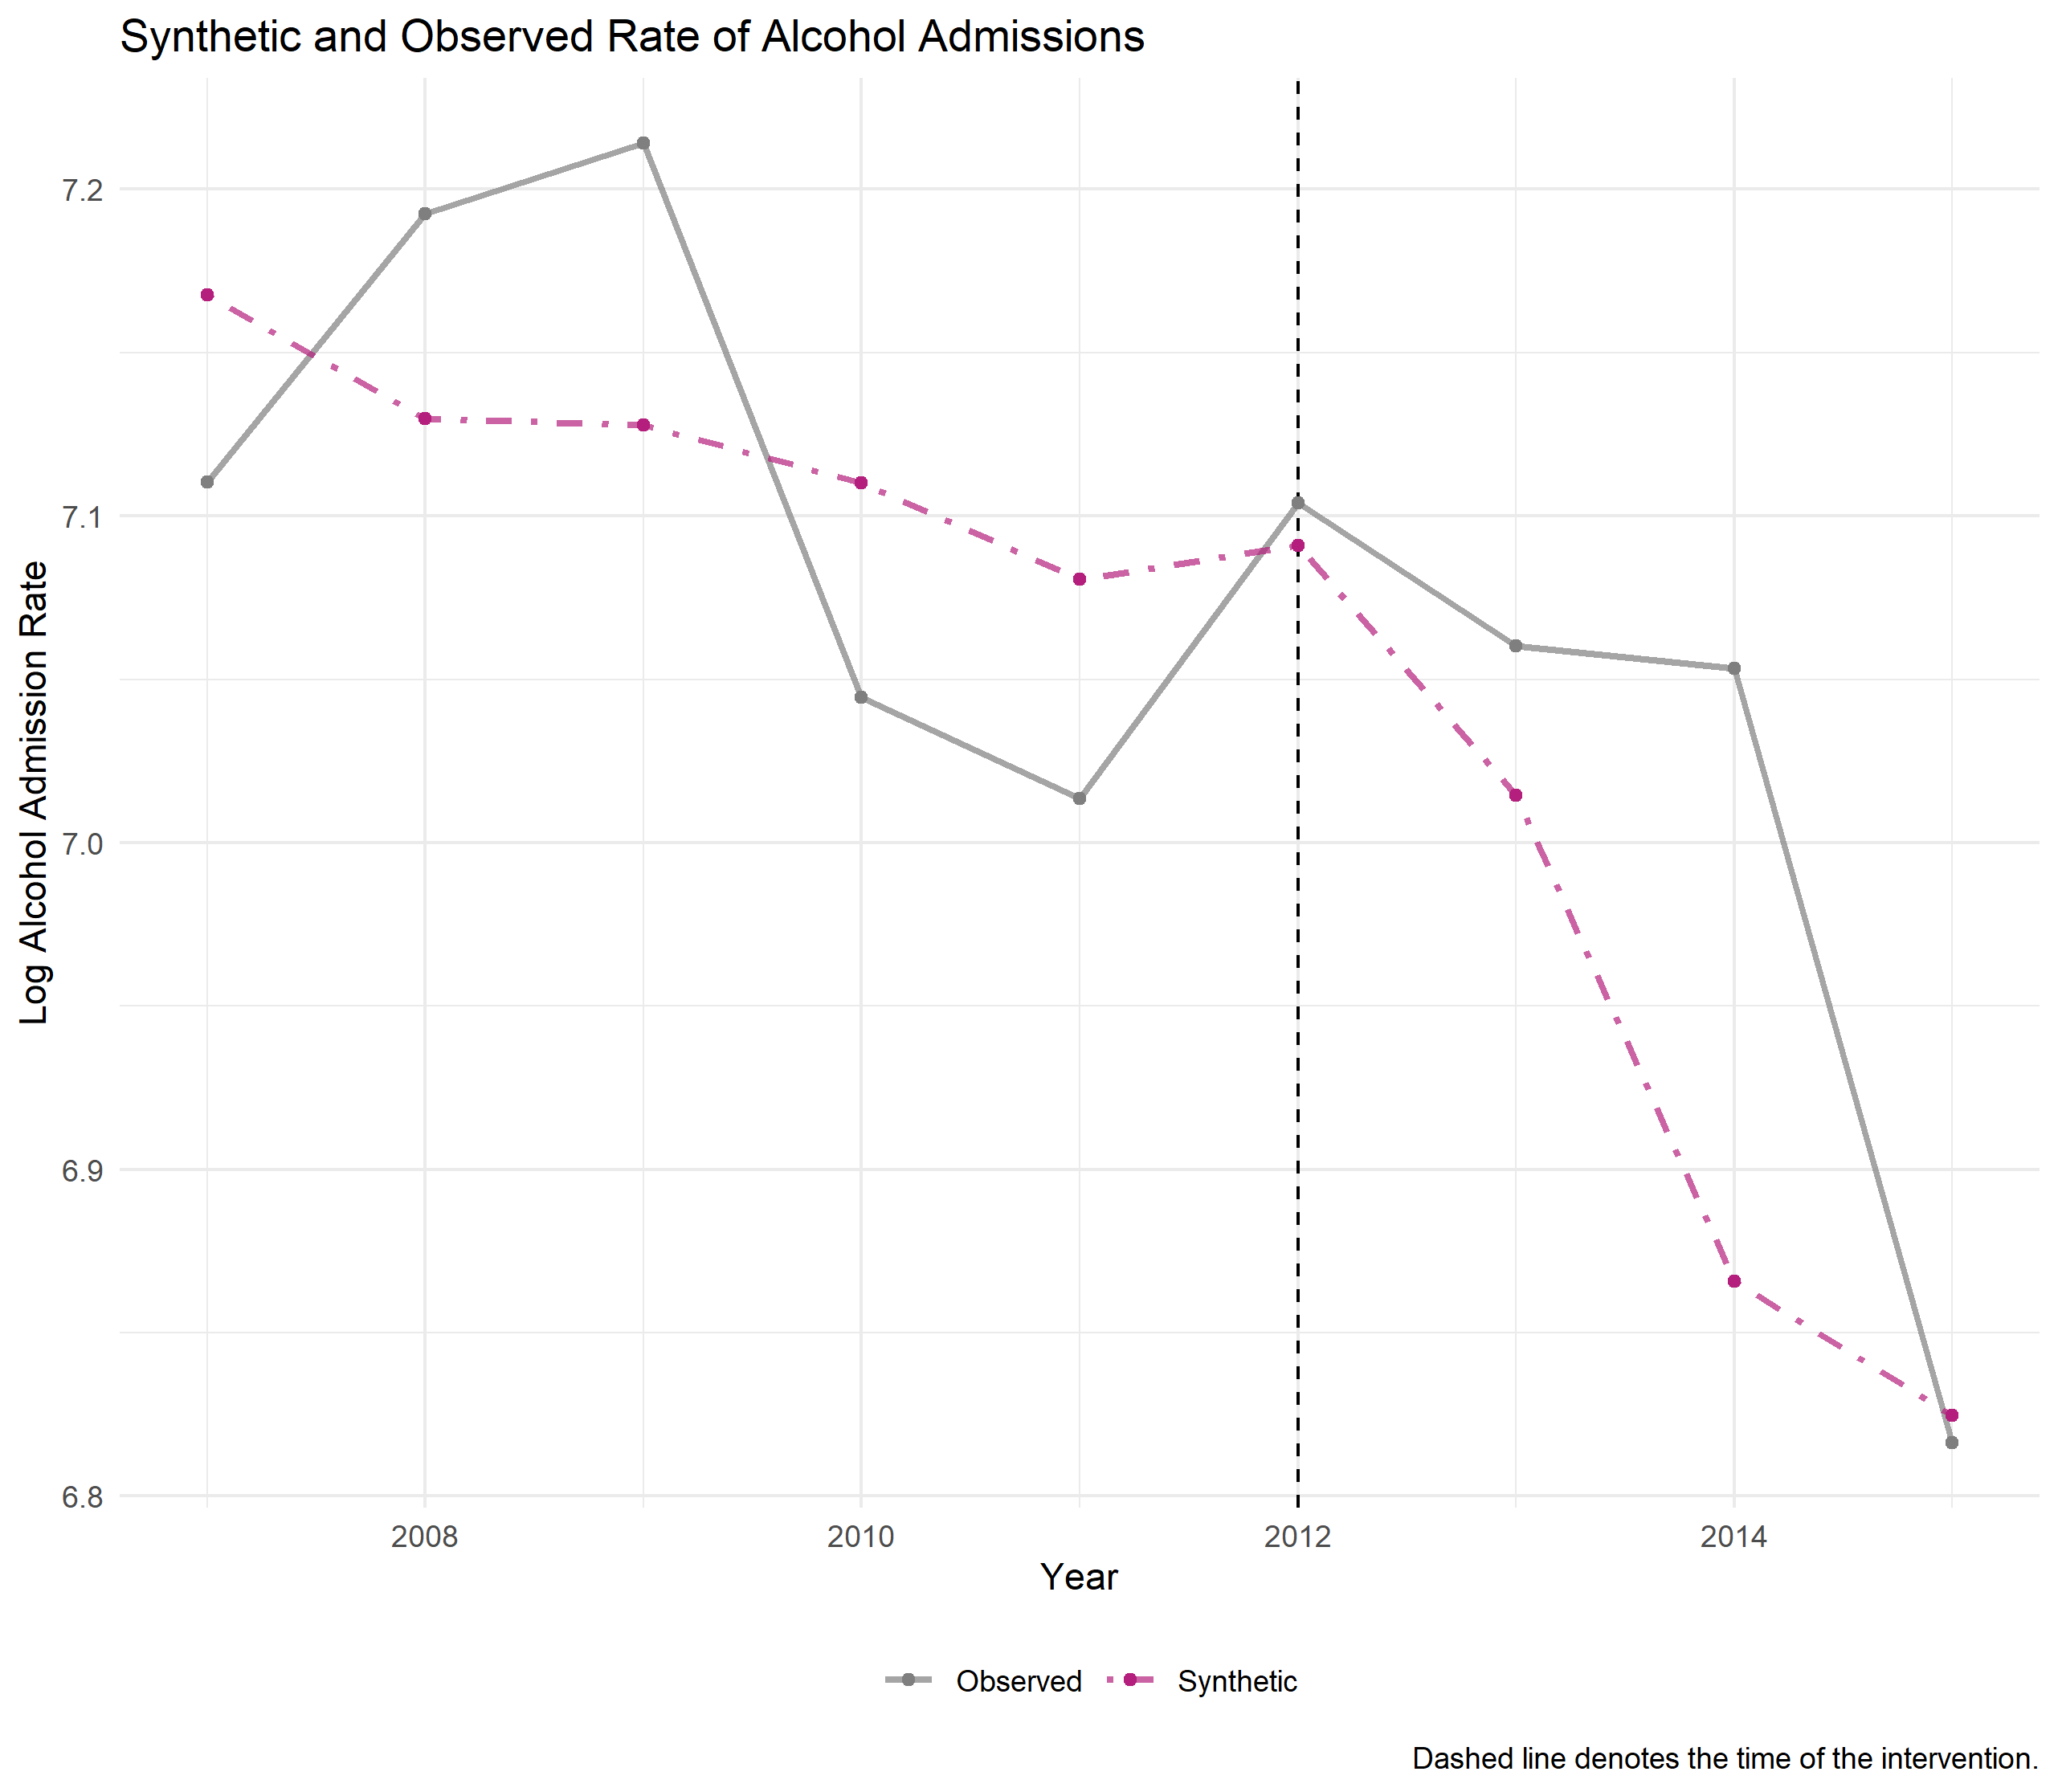
\includegraphics[width=.85\textwidth]{Figure_Trend_Alcohol.png}
    \end{center}
    \caption{Synthetic and Observed Rate of Alcohol Admissions by Year}
    \label{fig:AlcTrend}
\end{figure}

The effect on alcohol is entirely inconclusive; The data itself is very noisy, and the control is not a good predictor in the pre or the post group.

\begin{figure}[H]
    \begin{center}
        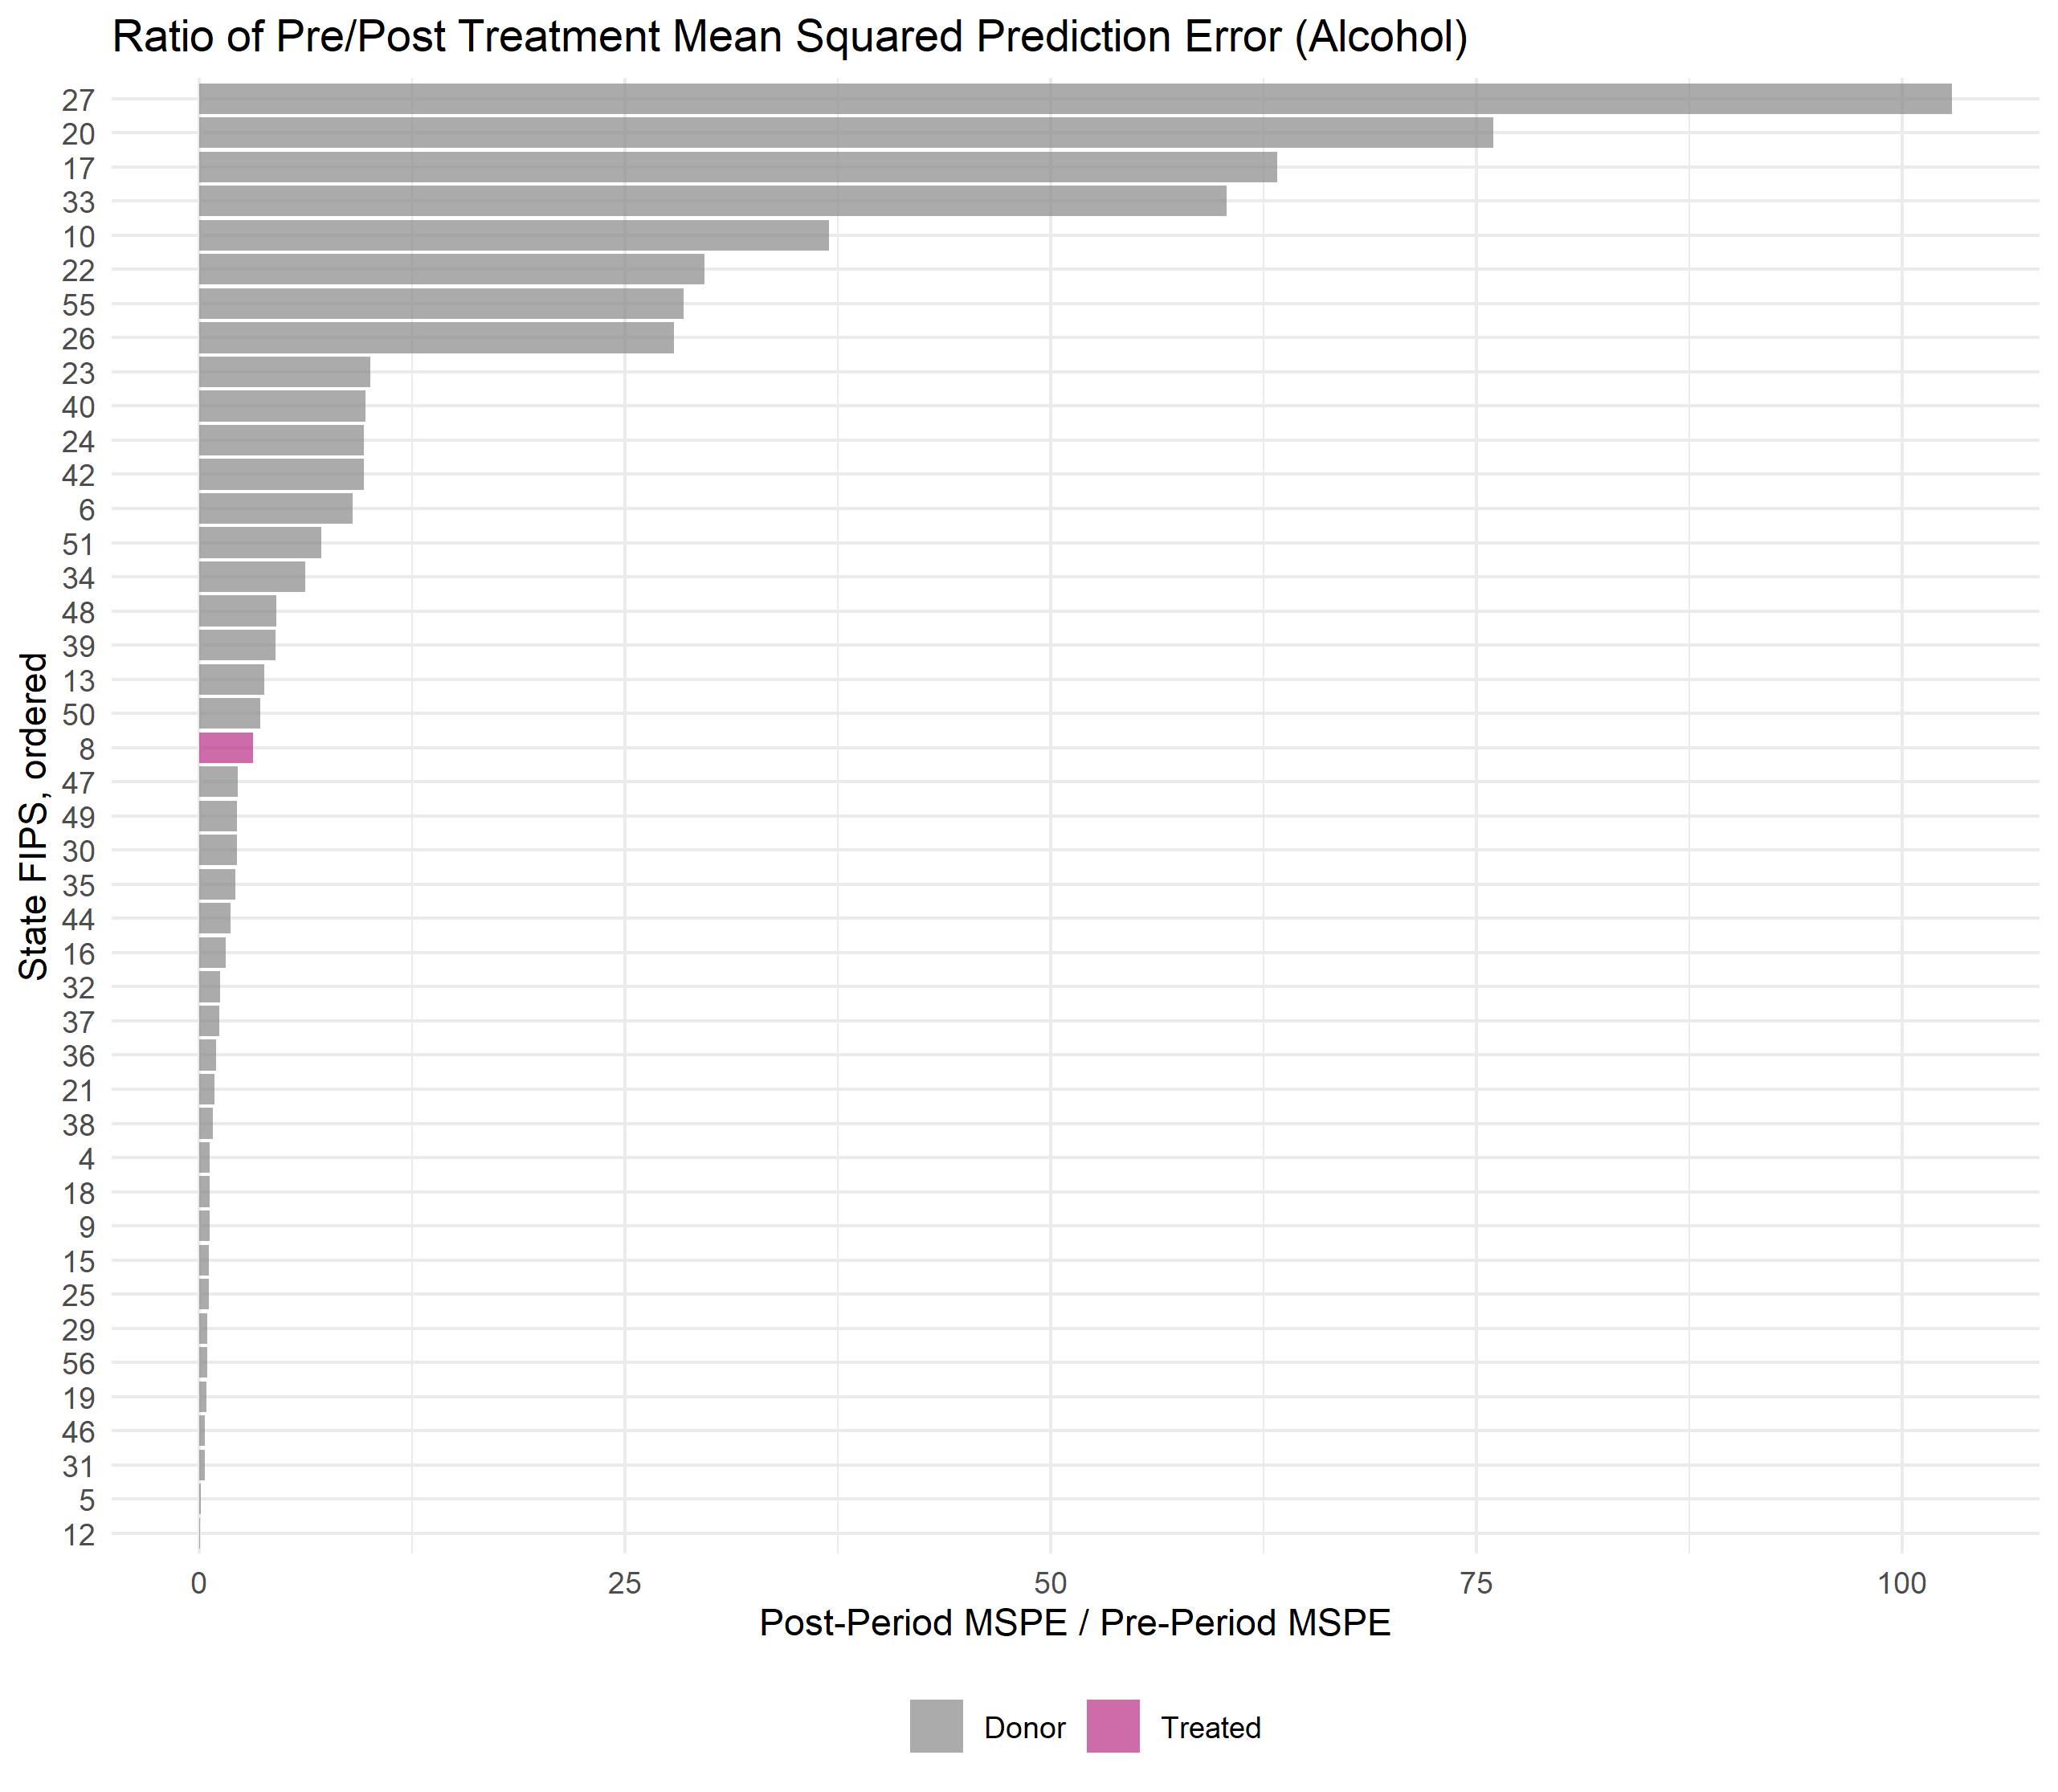
\includegraphics[width=.85\textwidth]{Figure_MSPERat_Alcohol.png}
    \end{center}
    \caption{Pre-Treatment to Post-Treatment MSPE Ratio: Alcohol}
    \label{fig:AlcMSPER}
\end{figure}

The issues carry through to our significance test, where we struggle to say that our results are statistically distinct from any of our placebo groups. This means simply that we cannot reject the null hypothesis that there was no effect of these laws on the rate of alcohol abuse.

This result is compelling since, intuitively, alcohol and marijuana would be the nearest substitutes in our data since they are both the 'mildest' substances and, post-legalization, the only pair that is completely legal. For this particular pair, the proposed substitution toward marijuana would be based on an underlying preference for marijuana over alcohol that, in the absence of deterrence, is now a more substantial factor. The failure to find any result here is the most notable failure to reject the null hypothesis.

\subsection*{Effect on Cocaine}

\begin{figure}[H]
    \begin{center}
        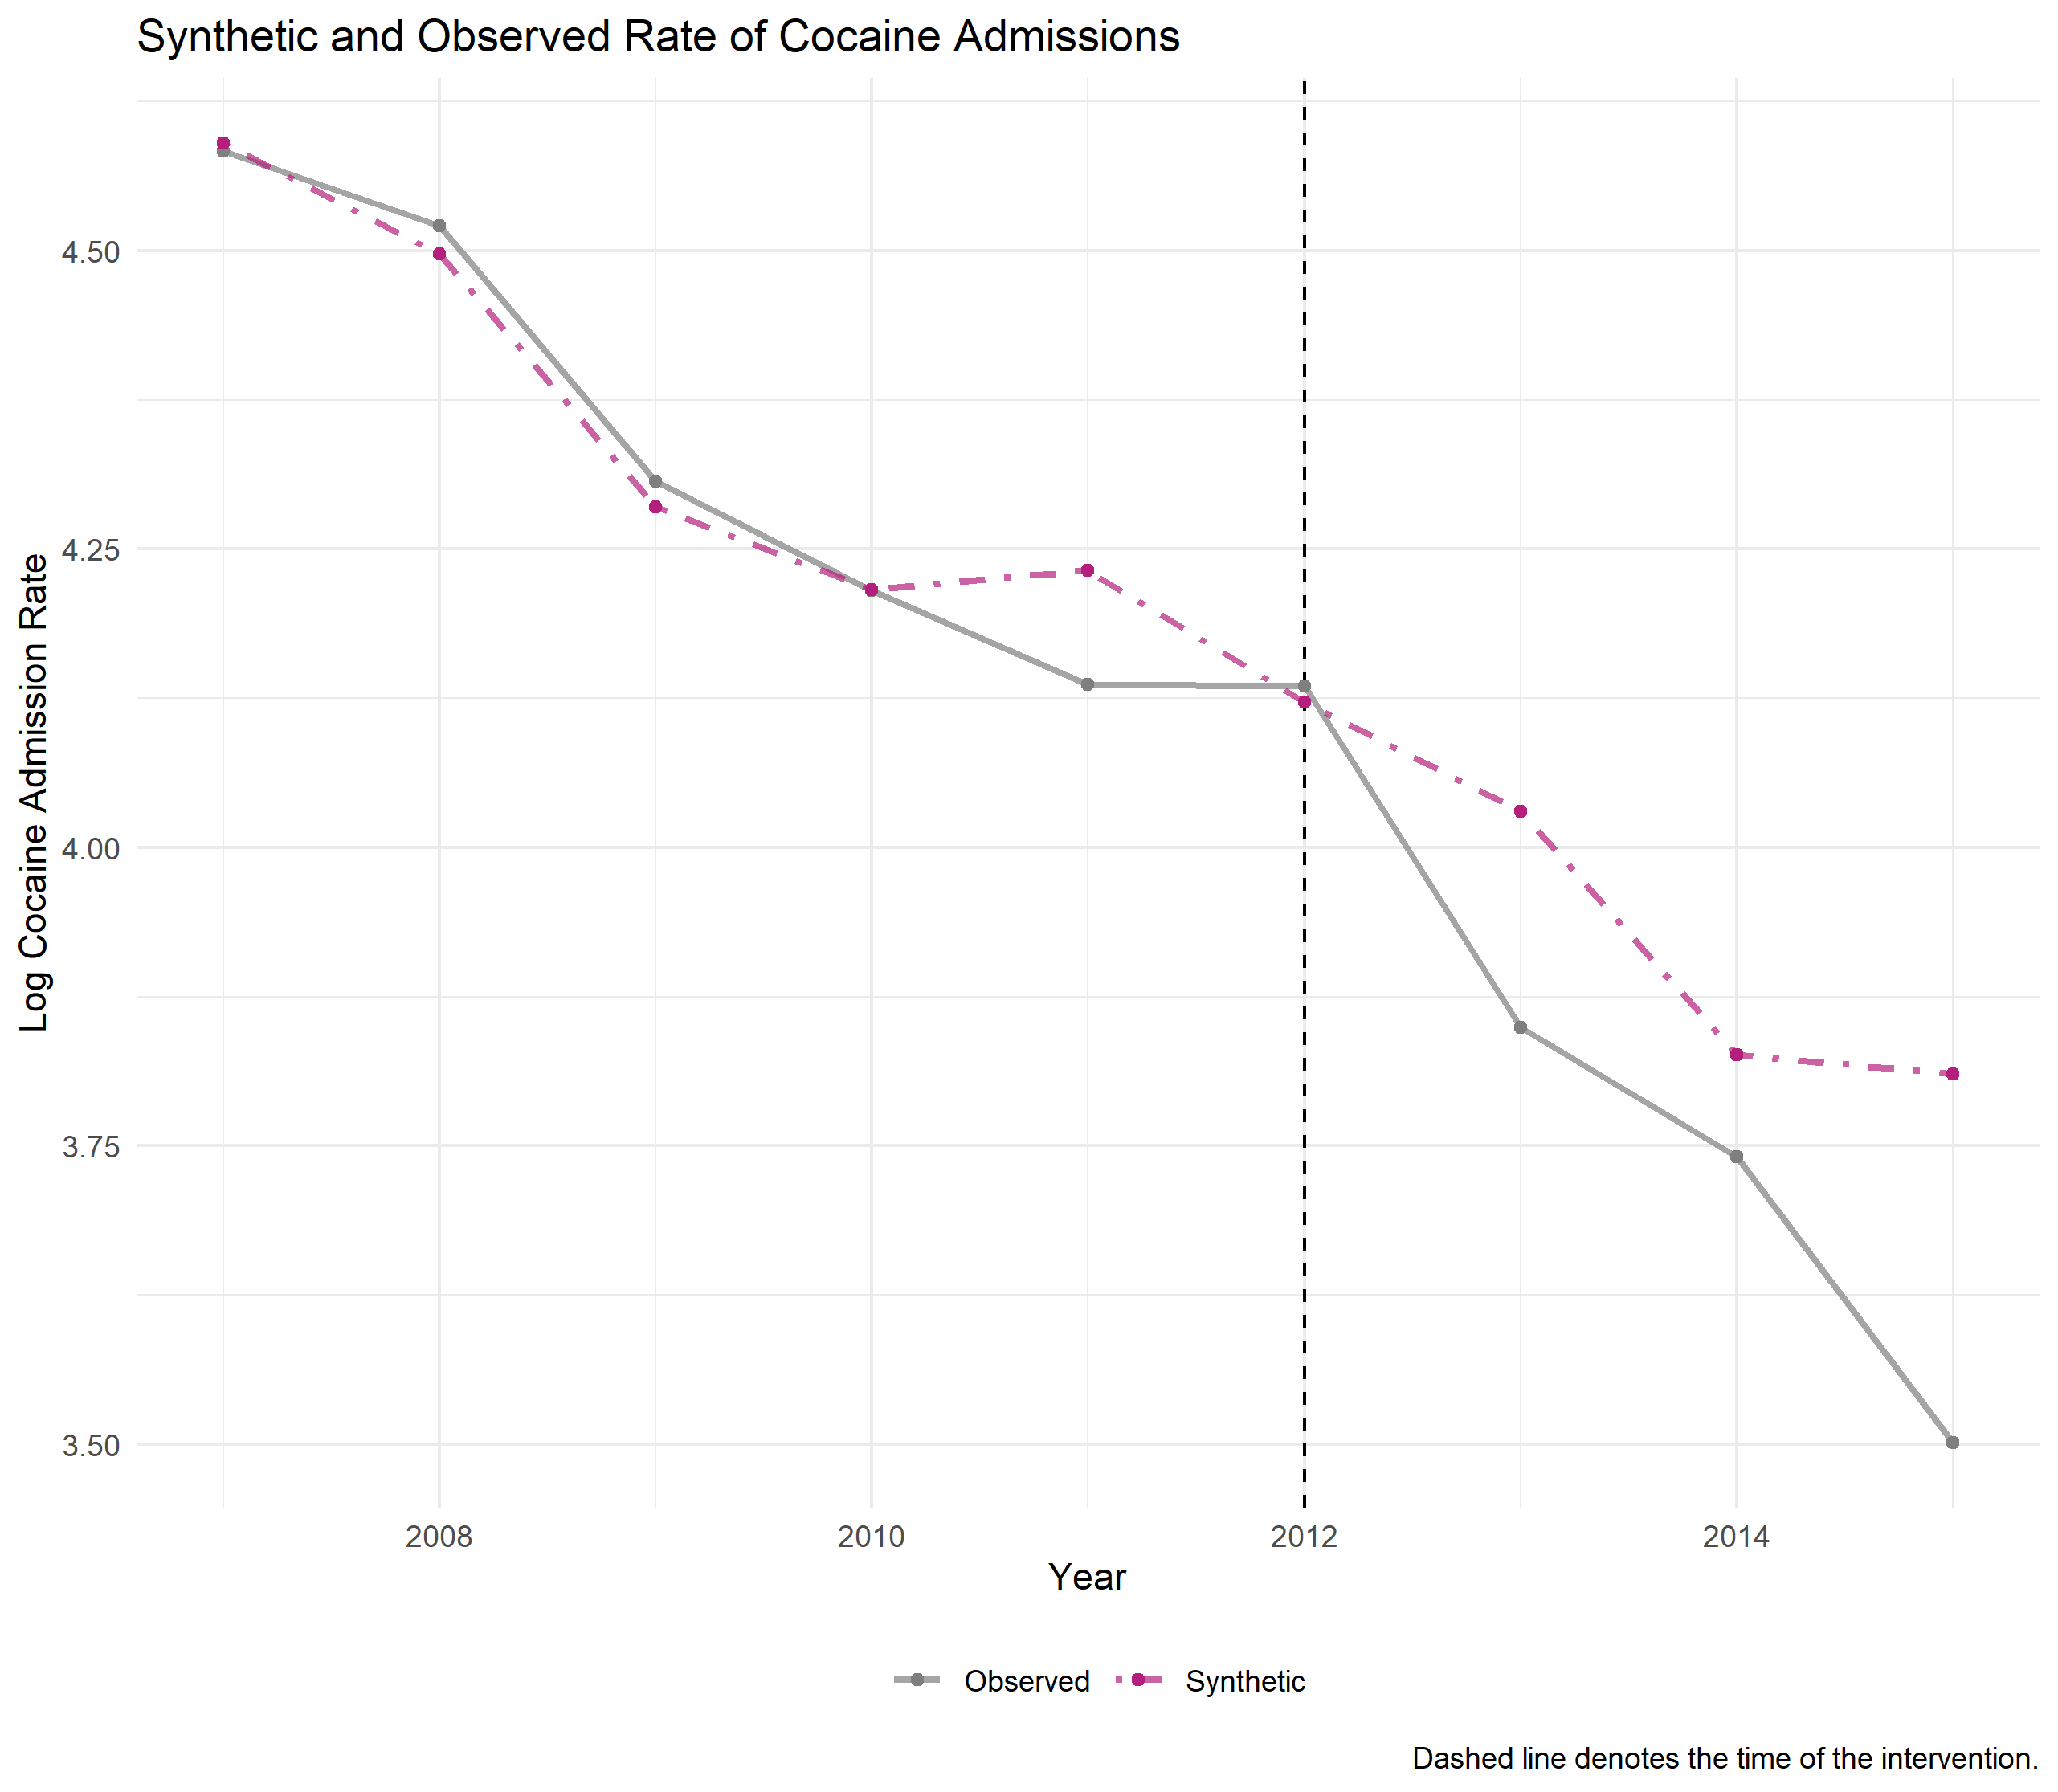
\includegraphics[width=.85\textwidth]{Figure_Trend_Cocaine.png}
    \end{center}
    \caption{Synthetic and Observed Rate of Cocaine Admissions by Year}
    \label{fig:CocTrend}
\end{figure}

The effect of legalization on cocaine is small, as seen in figure \ref{fig:CocTrend}, and statistically insignificant, as seen in figure \ref{fig:CocMSPER}. The main contrast of this outcome with alcohol is that the substitution from cocaine to marijuana has increased in value (theoretically) since marijuana no longer carries a harsh penalty for possession and use. If there were to be a substantial substitution toward marijuana based on a relative change in risk, a reduction in cocaine abuse would be expected. The lack of evidence here again detracts from the argument that these laws have much effect and suggests that \emph{much} more through studies would be required to provide concrete proof of their effect on cocaine.

\begin{figure}[H]
    \begin{center}
        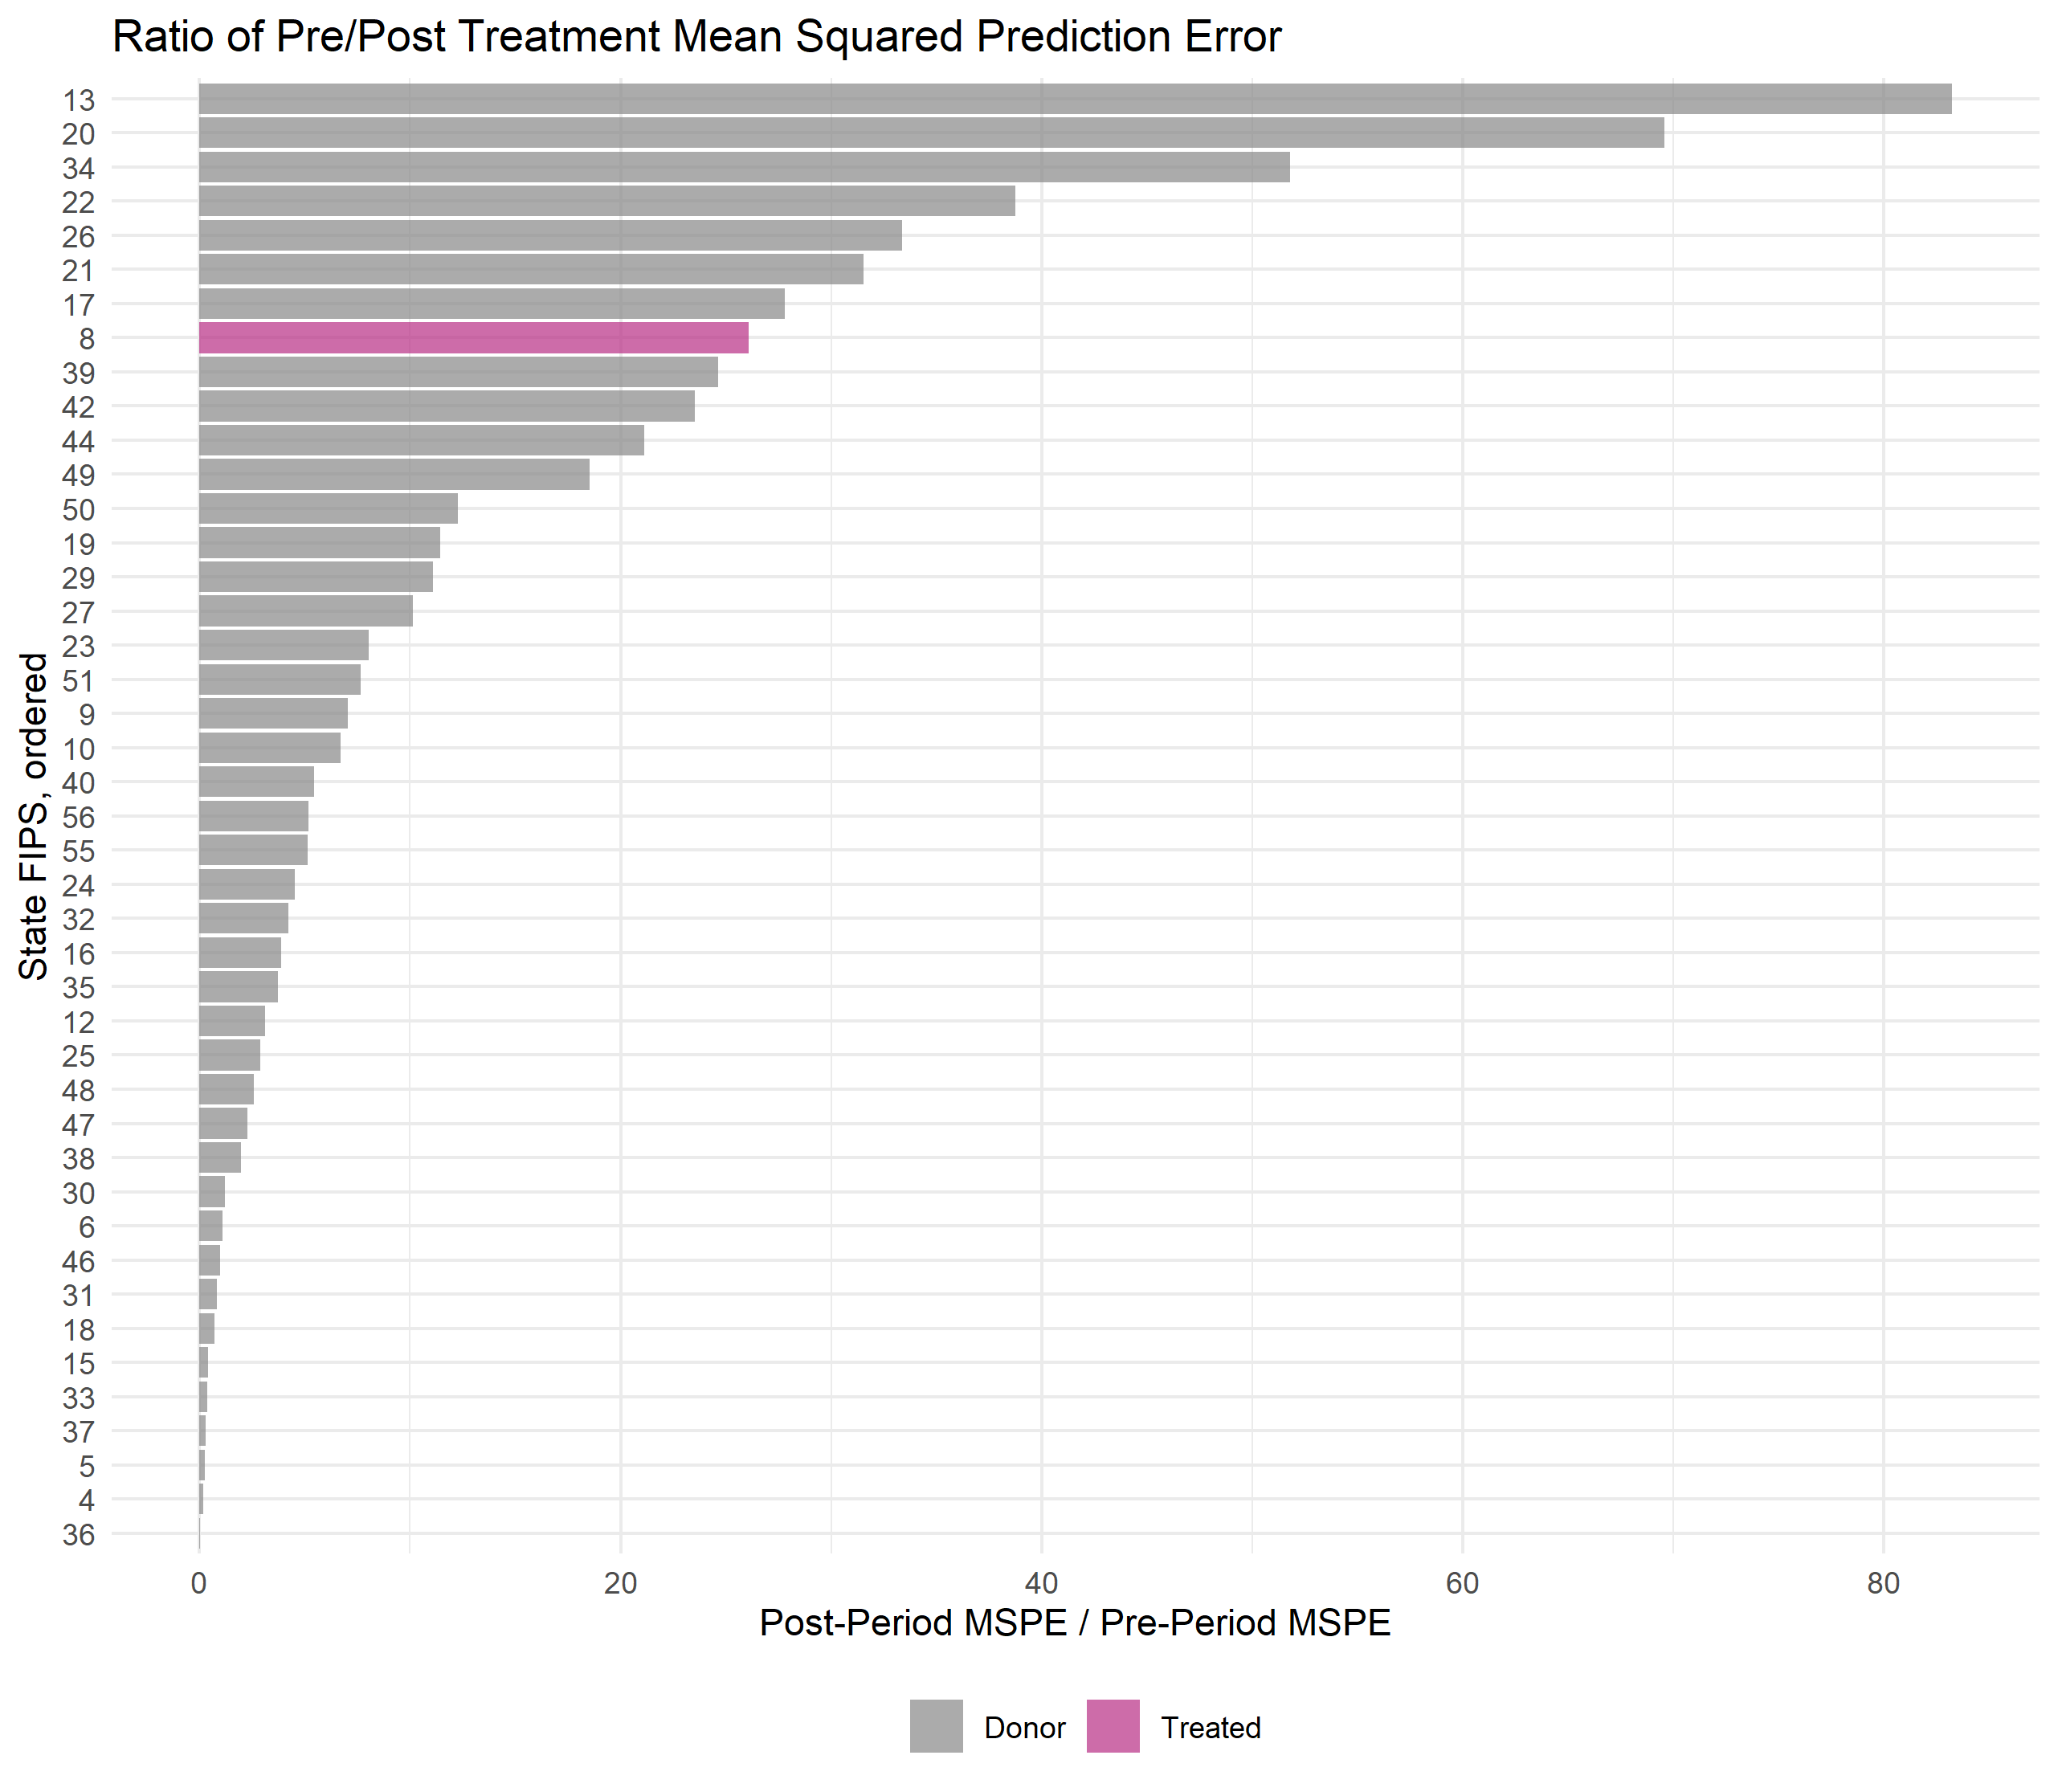
\includegraphics[width=.85\textwidth]{Figure_MSPERat_Cocaine.png}
    \end{center}
    \caption{Pre-Treatment to Post-Treatment MSPE Ratio: Cocaine}
    \label{fig:CocMSPER}
\end{figure}

\subsection*{Effect on Heroin}

We have substantially more data relating to the use of heroin across the country than any of the other drugs we investigate, which provides us with a clearer, more certain estimate.

\begin{figure}[H]
    \begin{center}
        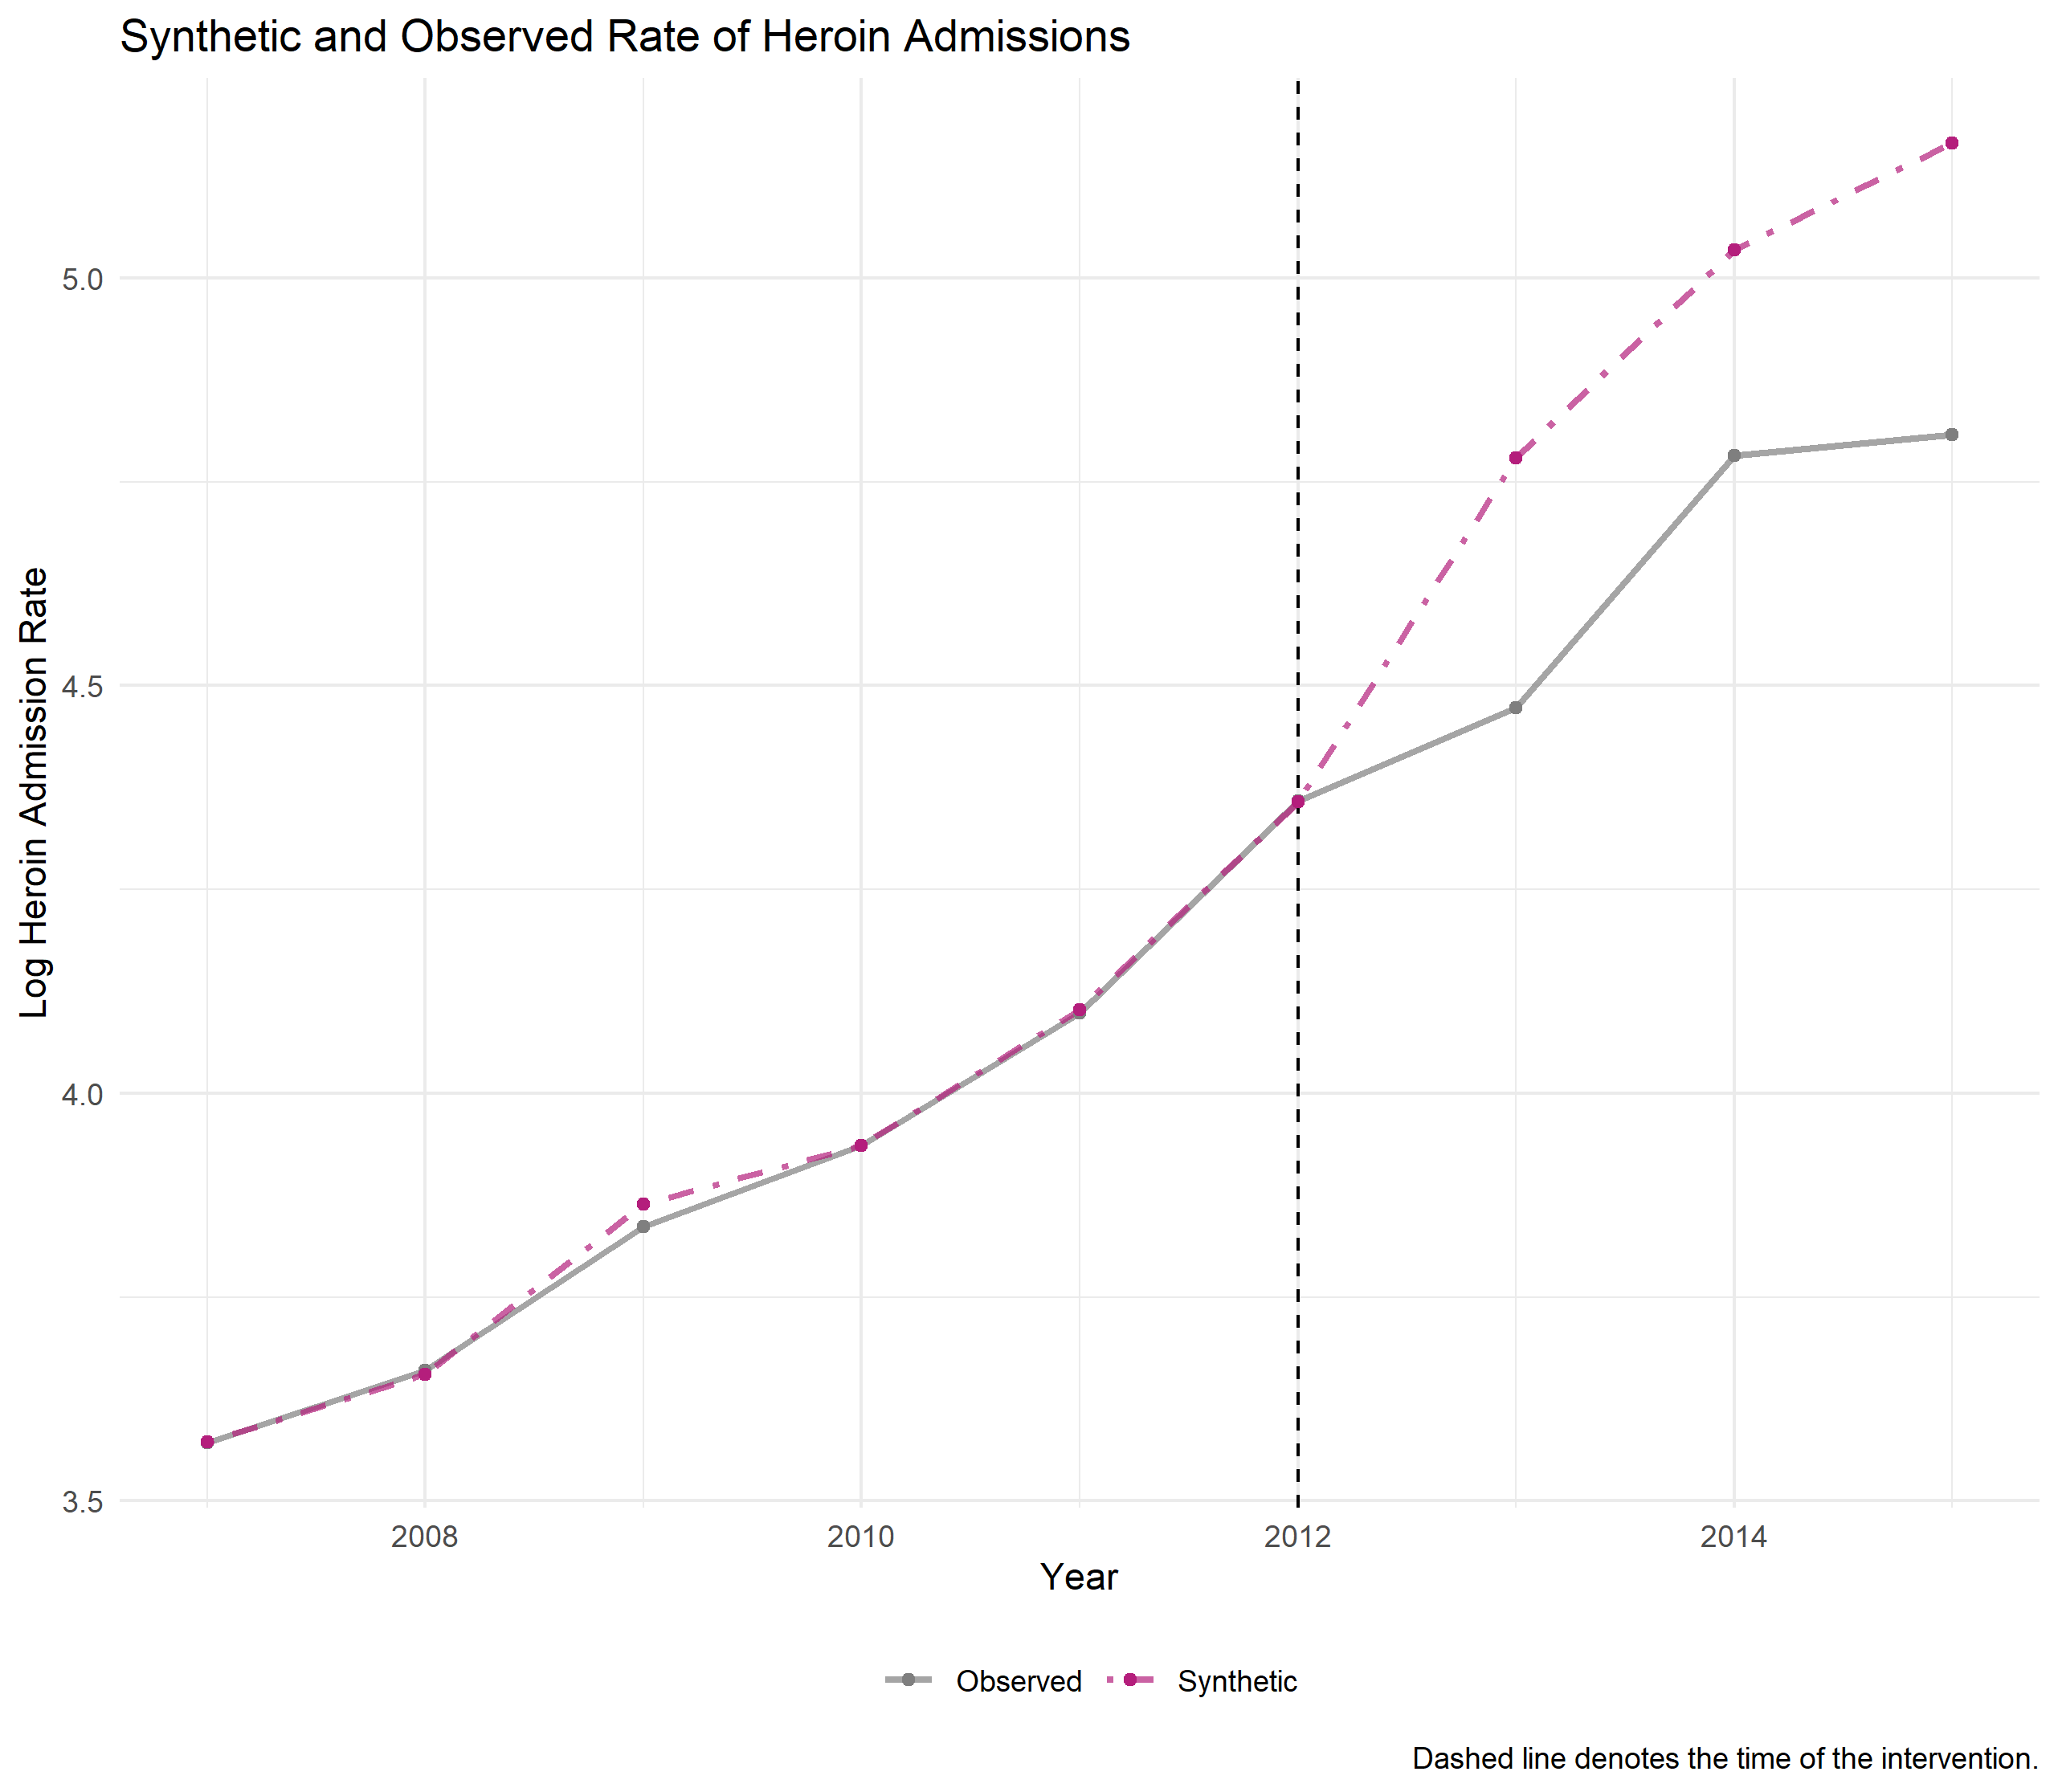
\includegraphics[width=.85\textwidth]{Figure_Trend_Heroin.png}
    \end{center}
    \caption{Synthetic and Observed Rate of Heroin Admissions by Year}
    \label{fig:HerTrend}
\end{figure}

The trend of this data is drastically different from the other drugs we consider: heroin is rapidly increasing, and we can say confidently here that the availability of legal marijuana reduces the rapid increase in abuse. 

\begin{figure}[H]
    \begin{center}
        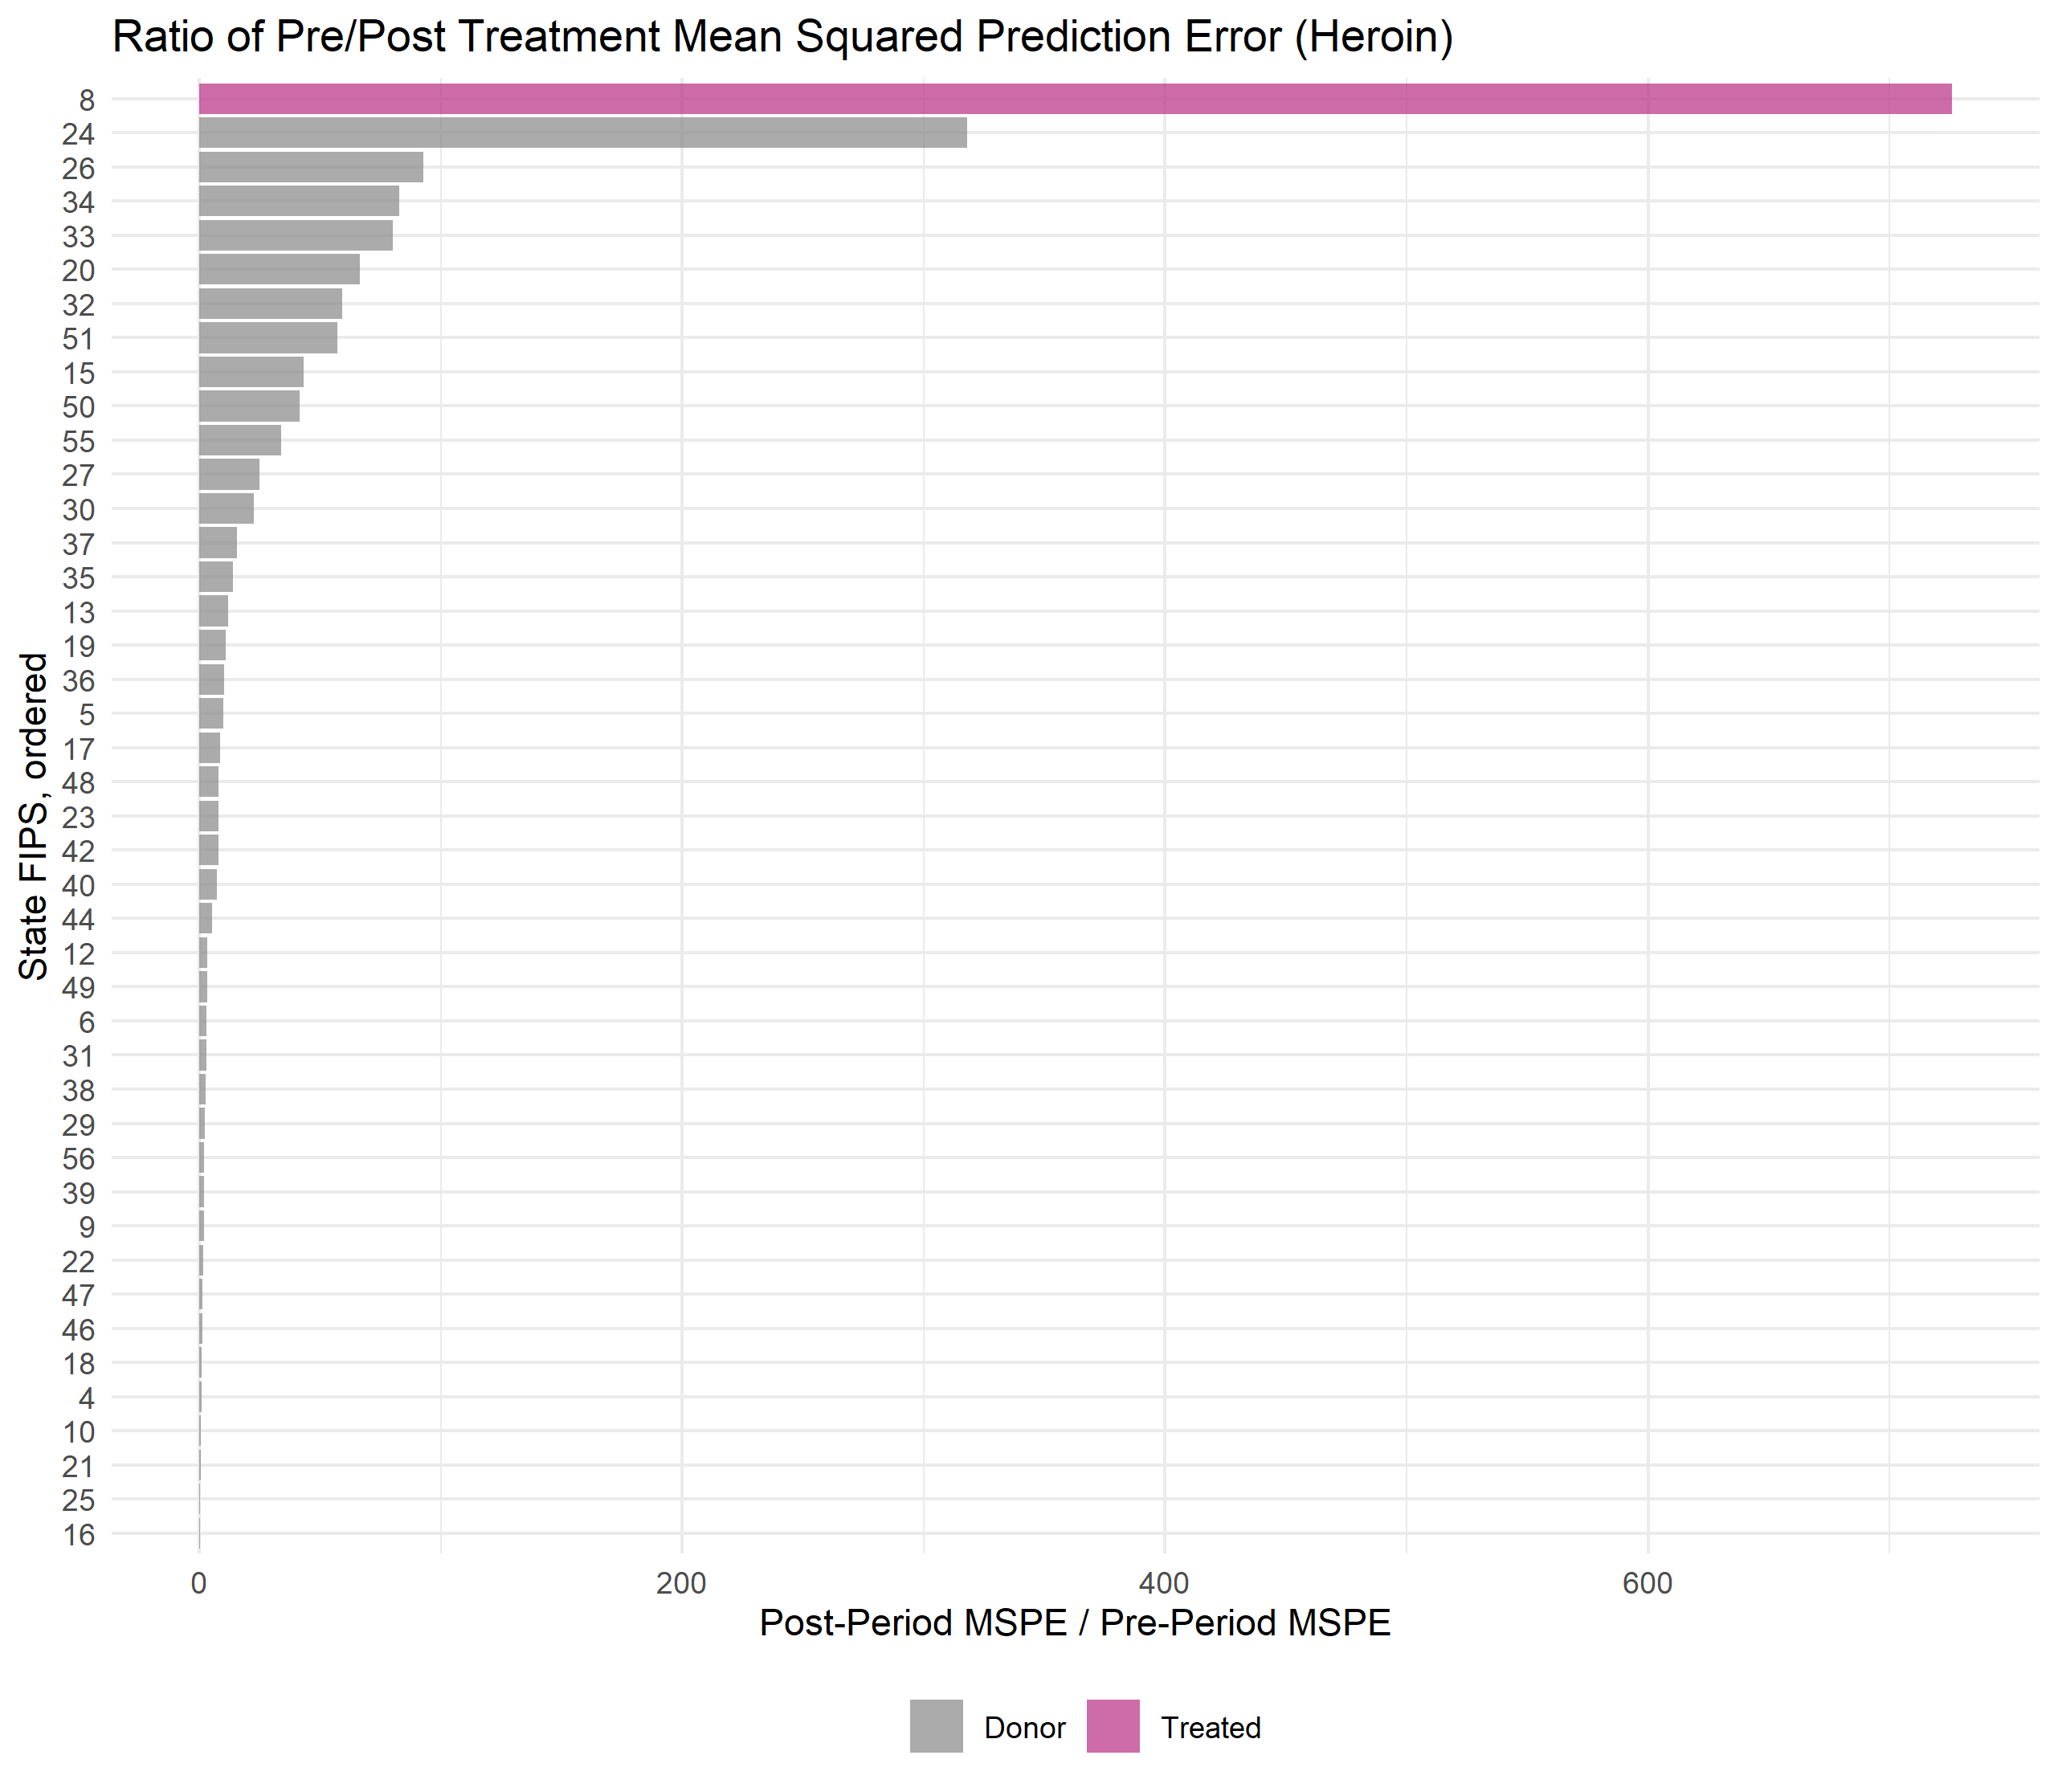
\includegraphics[width=.85\textwidth]{Figure_MSPERat_Heroin.png}
    \end{center}
    \caption{Pre-Treatment to Post-Treatment MSPE Ratio: Heroin}
    \label{fig:HerMSPER}
\end{figure}

The statistical significance here is undeniable; no placebo group has a ratio as large as the treatment group. According to the specification laid out by Abadie, Diamond, and Hainmueller \citeyearpar{SynthControl} the probability of finding a ratio this large, the Fisher sharp null, is $p=1/43 = 0.023 = 2.3\%$, which means we can fully reject the null hypothesis that this has no effect.

Looking closely at the balance of variables, we can see how close the synthesized data is to the observed data, and where it differs from the sample.

\begin{table}[!h]

\caption{\label{tab:BalTab}Balance of Variables in Treatment and Control}
\centering
\begin{tabular}[t]{lrrr}
\toprule
Variable & Colorado & Synthetic Colorado & Donor Sample\\
\midrule
\cellcolor{gray!6}{Mean Pop. Percent [18, 24]} & \cellcolor{gray!6}{0.0972454} & \cellcolor{gray!6}{0.0990390} & \cellcolor{gray!6}{0.0994441}\\
Mean Pop. Percent [25, 65] & 0.5497859 & 0.5434872 & 0.5269227\\
\cellcolor{gray!6}{Log Heroin Rate: 2007} & \cellcolor{gray!6}{3.5716798} & \cellcolor{gray!6}{3.5725237} & \cellcolor{gray!6}{3.2717930}\\
Log Heroin Rate: 2010 & 3.9361243 & 3.9355996 & 3.4594858\\
\cellcolor{gray!6}{Log Heroin Rate: 2012} & \cellcolor{gray!6}{4.3587951} & \cellcolor{gray!6}{4.3579199} & \cellcolor{gray!6}{3.7027434}\\
\bottomrule
\end{tabular}
\end{table}


The main difference is the vastly different rate of heroin use in 2012 between Colorado and the nationwide average. This could be for a number of reasons, but is clearly the important trend to have isolated in the data in order to properly estimate the counterfactual.

The final piece of intuition that is critical for our understanding are the placebo groups relative to the treatment group performance in the pre- and post-treatment period. Figure \ref{fig:HerPlac} is the only figure that reduces confidence in the results. There are no groups near to the treatment group in terms of pre-treatment accuracy. This does lessen the significance of the relatively-high MSPE ratio since it may indicate that the results are anomalous at the outlying value. However, given the high confidence in from our other metrics, this is a minor concern.

\begin{figure}[H]
    \begin{center}
        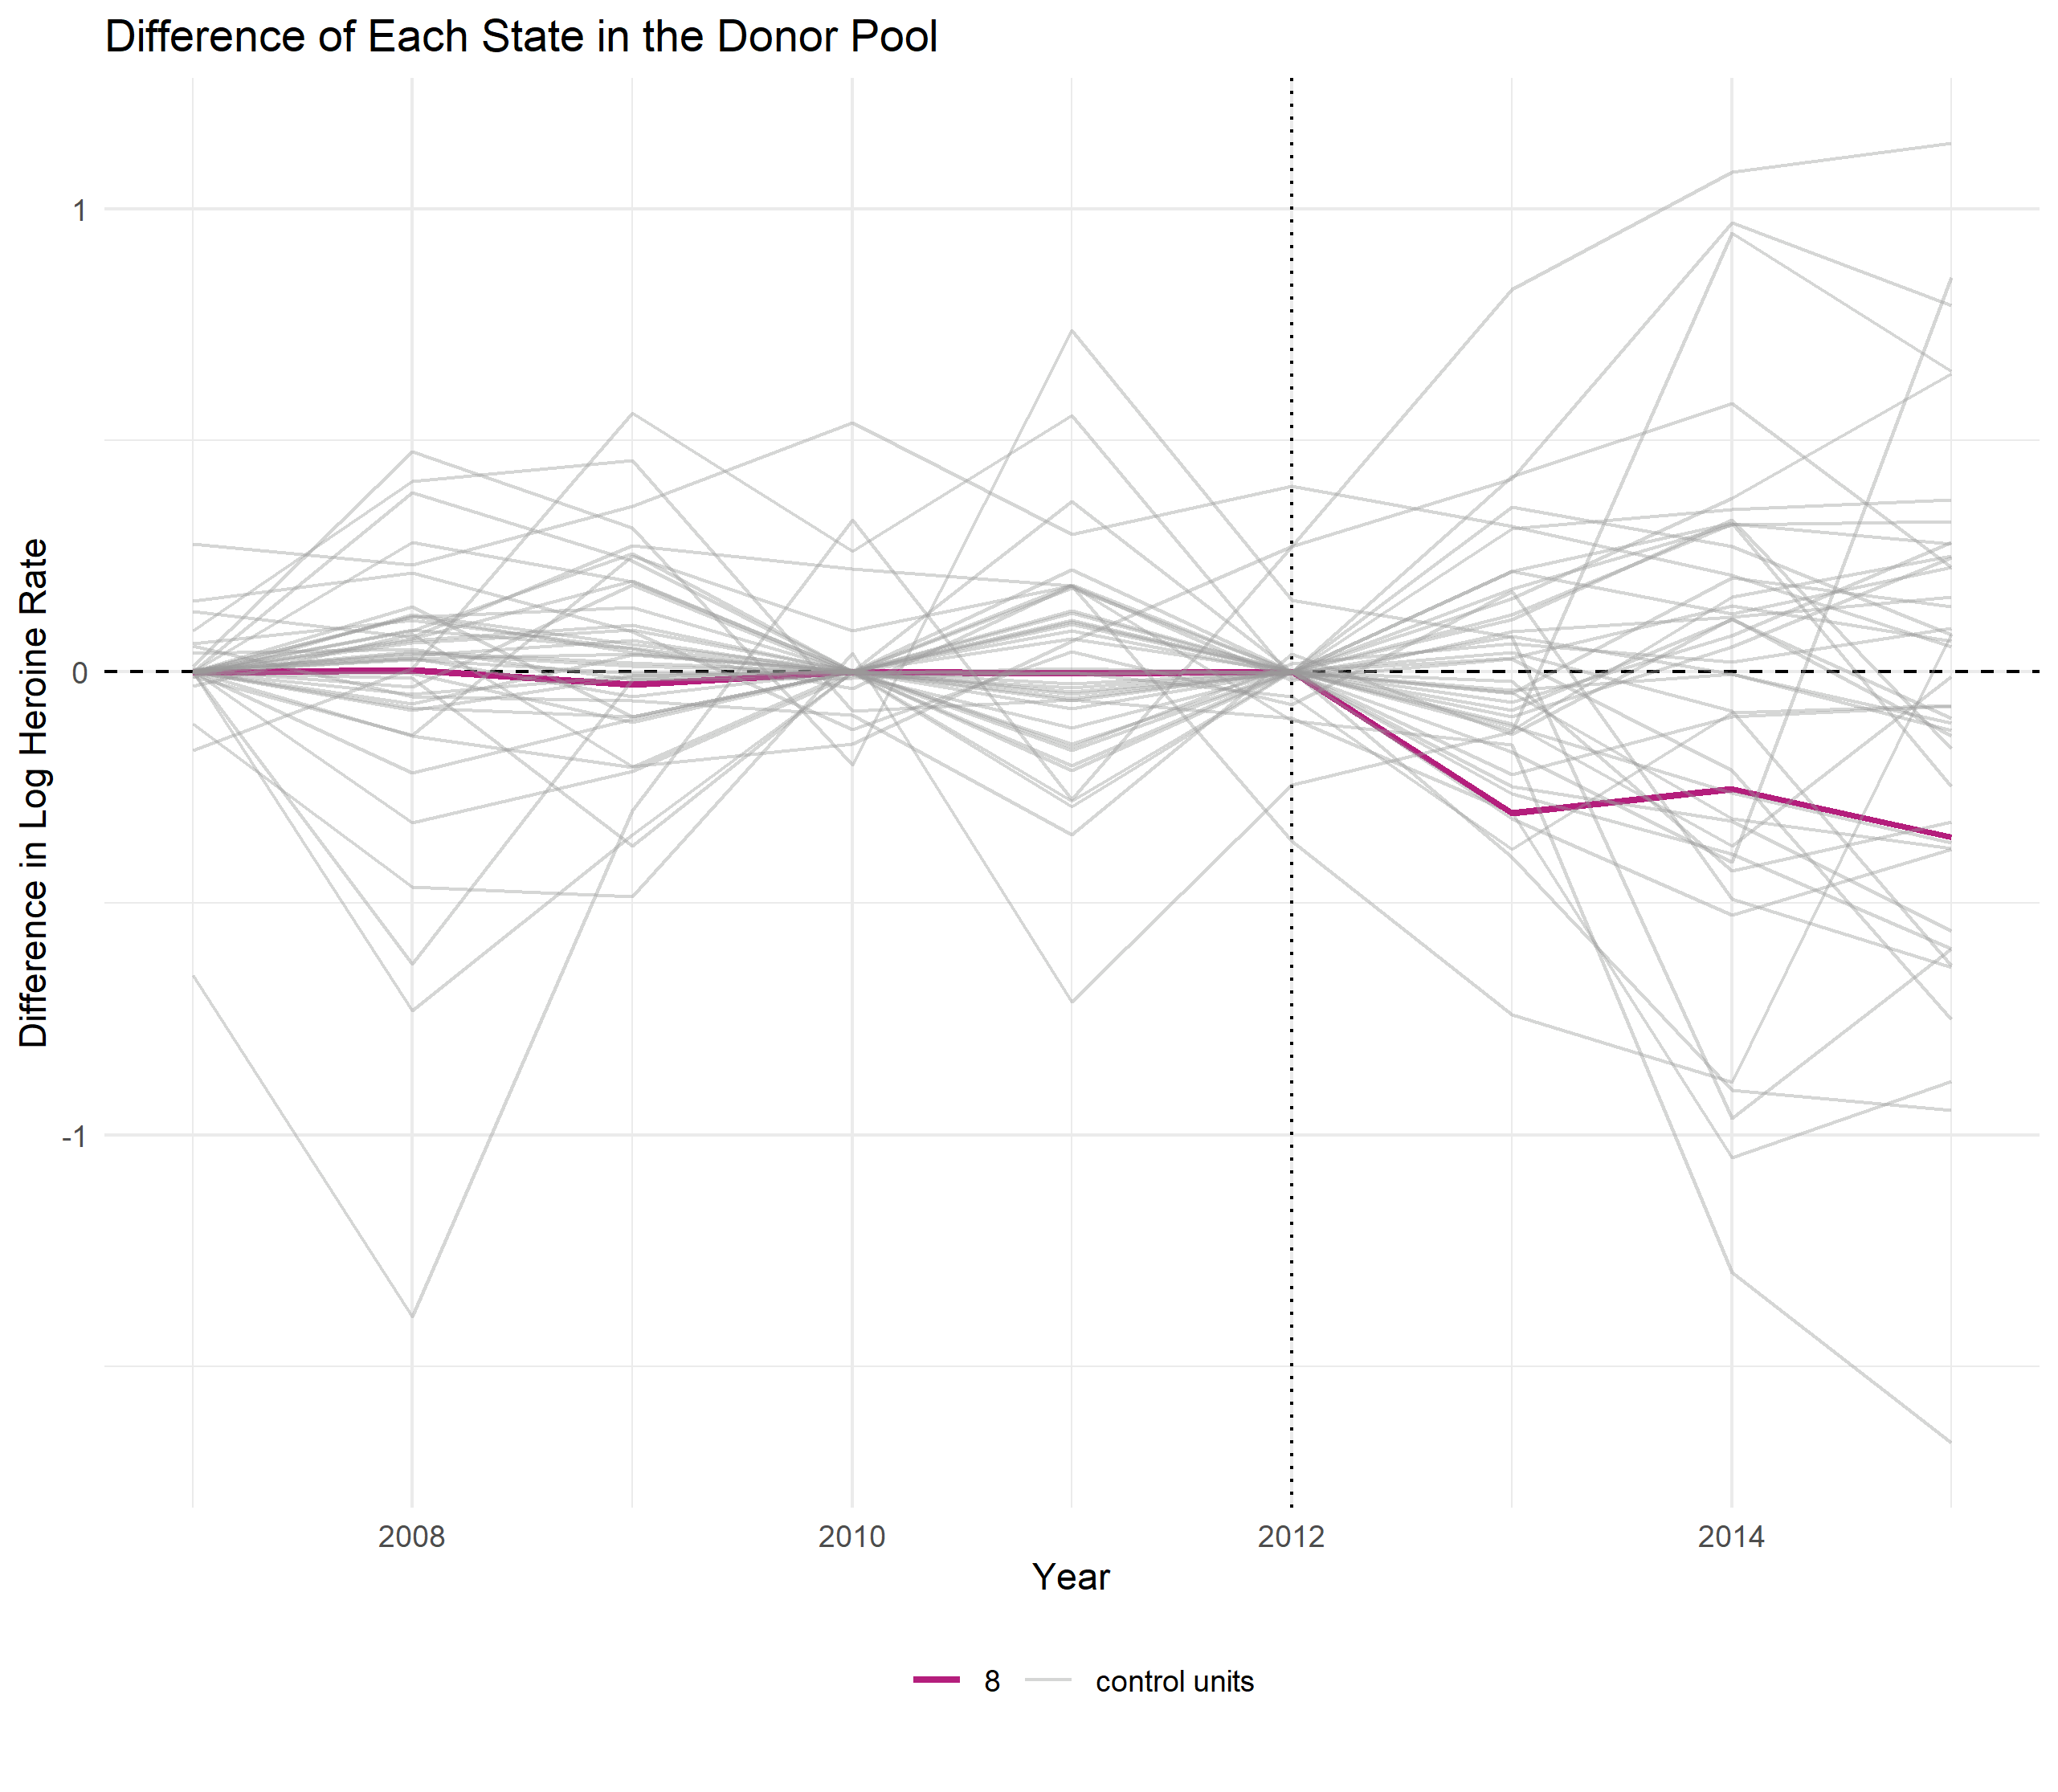
\includegraphics[width=.85\textwidth]{Figure_Placebos_Heroin.png}
    \end{center}
    \caption{Placebo Group Difference compared to Treatment Group Difference}
    \label{fig:HerPlac}
\end{figure}

\section{Conclusion}

The findings here indicate that the substantial effects of legalization are somewhat restricted to heroin but, given the exogenous observed trends in the data, this is hardly surprising. One limitation of our data that may explain some of this effect is that we are looking at admissions to treatment facilities, which includes intensive detox, intensive rehabilitation, and outpatient rehabilitation. Since the number of opiate users increases so much in our observed time period (and no others increased at all) it is probable that the reduction in heroin use are users that never began using heroin in the first place, rather than users that substituted away. Alcohol and cocaine addiction, on the other hand, is less likely to have begun during our time frame. Given the nature of addiction, it would be much more unlikely for these users to stop using a substance to which they were already addicted in favor of the now-legal marijuana.

The key takeaway from this analysis is that marijuana legalization may play a roll in reducing future abuse of addictive substances, with a limited effect on either accelerating or decelerating drugs that are already on downward trends.

This analysis also suggests further analysis on the total use of drugs (as opposed to late-stage treatment admissions) would be useful and, using similar methods, studying the link between legalization and medical-treatment efficiency may provide a deeper understanding of legalization and effective harm reduction.



\bibliography{LSC_Bib}
\bibliographystyle{apalike}

\end{document}